\documentclass[aspectratio=169]{beamer}

\definecolor{myaccent}{HTML}{356AE6}
\usetheme[
  accent=myaccent,
  progressbar=none,
  sectionpage=simple,
  subsectionpage=none,
  numbering=fraction,
  titleformat=regular,
  block=fill
]{cookie}

% Render equations in the classic serif math font (Latin Modern / Computer
% Modern) instead of the theme's sans-serif default. [onlymath] leaves the
% body text in Fira Sans and only affects math.
\usefonttheme[onlymath]{serif}

% Override Cookie's section divider so it also lists the section's subsections
% as sub-points. This keeps the theme file pristine; it copies the theme's
% section page and adds a \tableofcontents[currentsection] node (subsections
% only) below the title. \cookie@format / colors are the theme's own macros.
\makeatletter
\setbeamertemplate{subsection in toc}{%
  \leavevmode\leftskip=2em\rlap{\raise.05ex\hbox{\textbullet}}\hskip1em%
  \inserttocsubsection\par%
}
\renewcommand{\cookie@sectionpageframe}{%
  \begin{frame}[plain,noframenumbering,c]
    \begin{tikzpicture}[remember picture,overlay]
      \fill[cookieAccent]
        (current page.south west) rectangle ($(current page.north west)+(.012\paperwidth,0)$);
      \node[anchor=west,text=cookieAccent,font=\fontsize{46}{46}\selectfont\bfseries]
        at ($(current page.west)+(.07\paperwidth,.22\paperheight)$) {\insertsectionnumber};
      \node[anchor=west,text width=.80\paperwidth,align=left]
        at ($(current page.west)+(.07\paperwidth,.10\paperheight)$)
        {{\usebeamerfont{section title}\usebeamercolor[fg]{section title}\cookie@format{\insertsection}}};
      \node[anchor=north west,text width=.80\paperwidth,align=left]
        at ($(current page.west)+(.07\paperwidth,-.04\paperheight)$)
        {\begin{minipage}{.80\paperwidth}%
           \fontsize{14}{16}\selectfont\usebeamercolor[fg]{normal text}%
           \tableofcontents[currentsection,%
             sectionstyle=hide/hide,%
             subsectionstyle=show/show/hide]%
         \end{minipage}};
      \fill[cookieAccent] ($(current page.east)+(-.095\paperwidth,.24\paperheight)$) circle[radius=.014\paperheight];
      \fill[cookieAccent,opacity=.45] ($(current page.east)+(-.072\paperwidth,.18\paperheight)$) circle[radius=.008\paperheight];
    \end{tikzpicture}
  \end{frame}%
}
\makeatother

% Shared bibliography with the thesis: natbib + BibTeX (apj style), pointing at
% thesis/references.bib. build.sh puts thesis/ on BIBINPUTS/BSTINPUTS so the
% .bib and apj.bst are found without copying them here.
\usepackage[numbers,sort&compress]{natbib}
\usepackage{booktabs}

\title{Radio Recombination Line Forecasts with CHORD}
\author{Duncan Cameron-Steinke\\ \\ Supervisor: Dr. Alex Hill}
\date{\today}

\begin{document}
\maketitle

\makeagenda

\section{Background}

\subsection{The Interstellar Medium}
\begin{frame}{The Interstellar Medium (ISM)}{}
  \begin{columns}[T]
    \begin{column}{0.5\linewidth}
      \begin{itemize}
        \item The ISM is the gas and dust between stars.
        \item The ISM traces the structure of the Milky Way, providing information on Galactic evolution, star formation, and more.
        \item 70\% of the ISM is hydrogen, which can be detected through H$\alpha$ emission.
      \end{itemize}
    \end{column}
    \begin{column}{0.5\linewidth}
      \centering
      {\usebeamercolor[fg]{structure}Wisconsin H$\alpha$ Mapper sky survey}
      \par\smallskip
      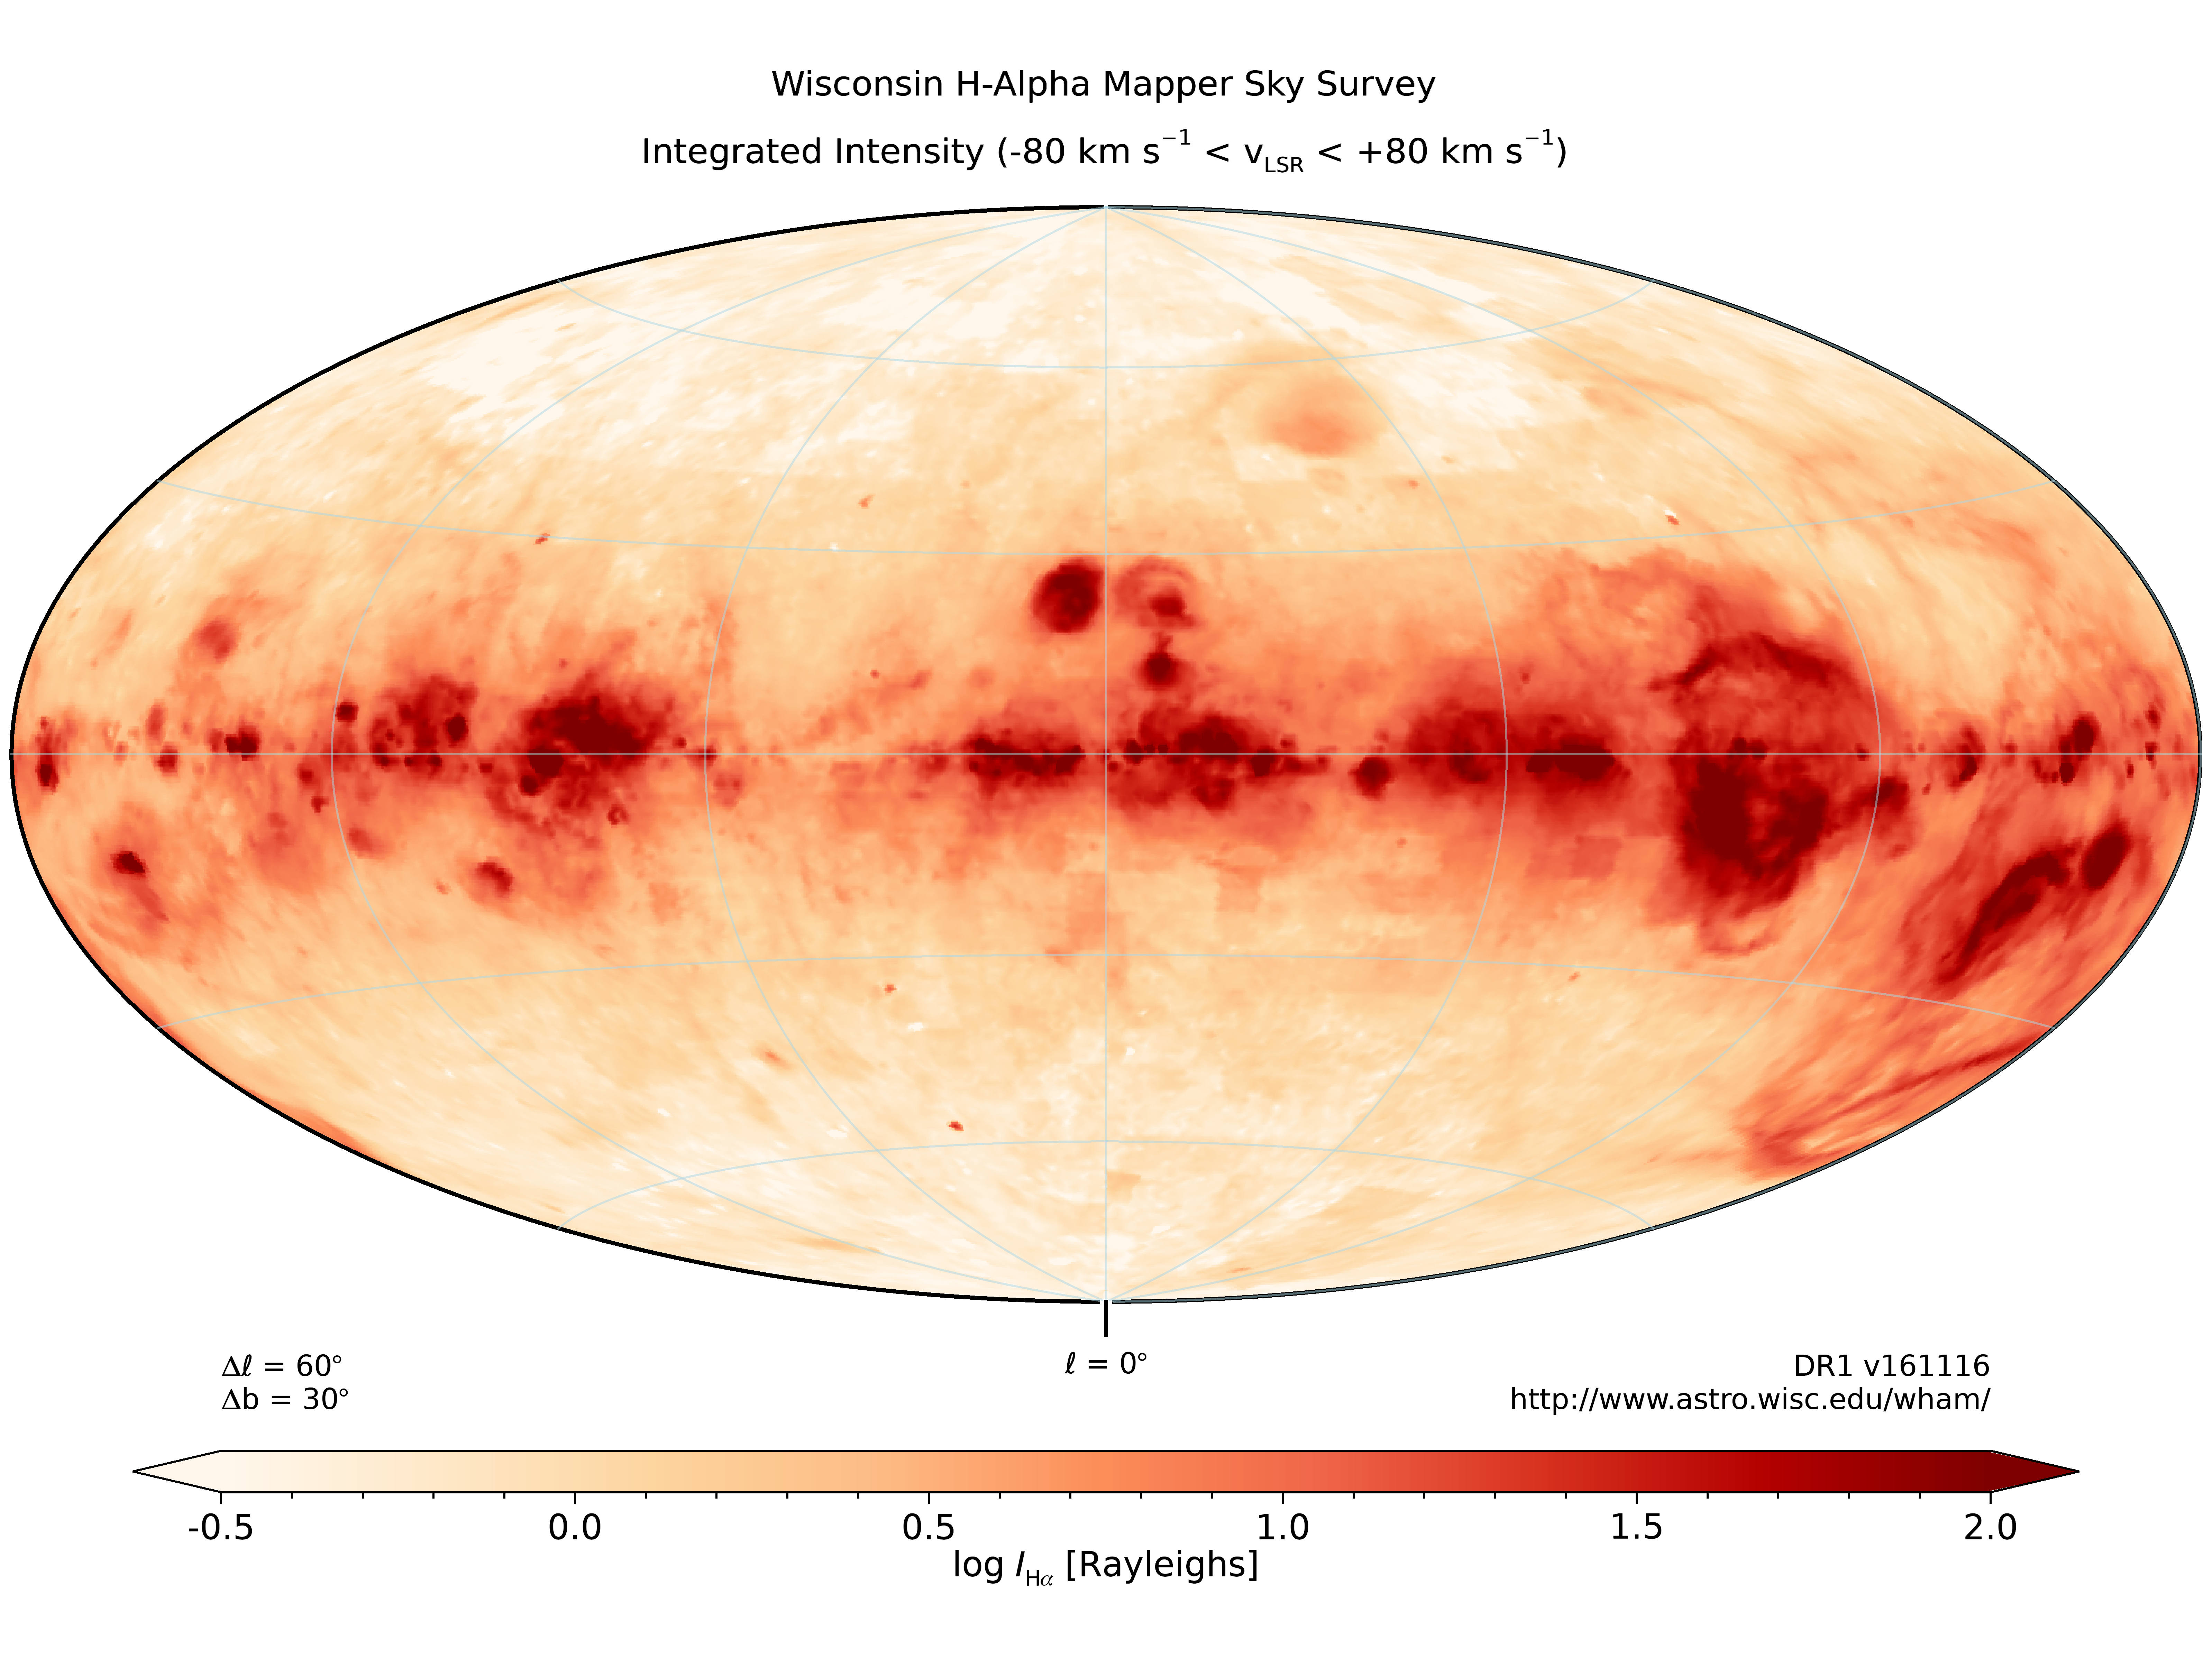
\includegraphics[width=0.8\linewidth]{plots/wham_image.png}
      \par\medskip
      {\footnotesize All-sky map of H$\alpha$ emission in the visible spectrum \cite{haffnerEarlyResultsWisconsin2010}.}
    \end{column}
  \end{columns}
\end{frame}

\subsection{Radio Recombination Lines}
\begin{frame}{Radio Recombination Lines (RRLs)}{}
  \begin{columns}[T]
    \begin{column}{0.5\linewidth}
      \begin{itemize}
        \item Hot stars ionize the ISM, when the ionized electrons recombine with protons, they cascade through atomic energy levels, emitting photons at each transition.
        \item These photons can be detected on earth to measure the properties of the ISM.
        \item Radio recombination lines (RRLs) specifically refer to the radio emission from these transitions.
      \end{itemize}
    \end{column}
    \begin{column}{0.4\linewidth}
      \centering
      {\usebeamercolor[fg]{structure}Bohr atomic model}
      \par\smallskip
      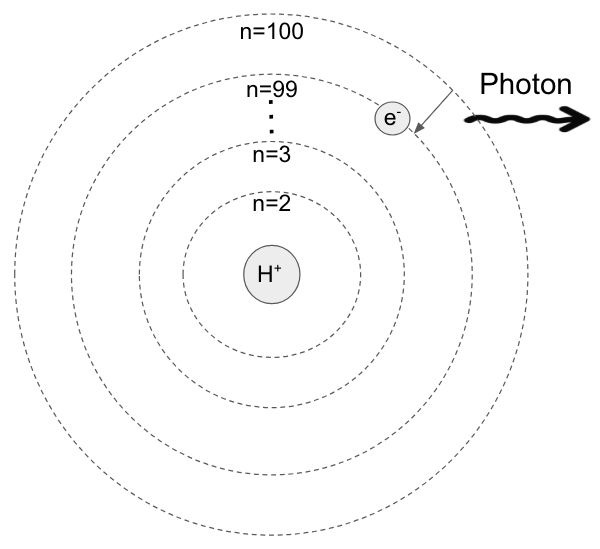
\includegraphics[width=0.8\linewidth]{plots/rrl_model.png}
      \par\medskip
      {\footnotesize Simplified Bohr model of the hydrogen atom showing RRL emission from $N=100 \to 99$.}
    \end{column}
  \end{columns}
\end{frame}

\subsection{CHORD}
\begin{frame}{The Canadian Hydrogen Observatory and Radio-transient Detector (CHORD)}{}
  \begin{columns}[T]
    \begin{column}{0.5\linewidth}
      \begin{itemize}
        \item CHORD is a radio interferometer being constructed at the Dominion Radio Astro-physical Observatory (DRAO) in British Columbia, Canada.
        \item CHORD can observe frequencies from 300 MHz to 1.5 GHz, which encompasses 116 Hn$\alpha$ RRLs.
        \item The goal of this research is to assess the performance of using CHORD for RRL observations of the ISM.
      \end{itemize}
    \end{column}
    \begin{column}{0.4\linewidth}
      \centering
      {\usebeamercolor[fg]{structure}CHORD under construction}
      \par\smallskip
      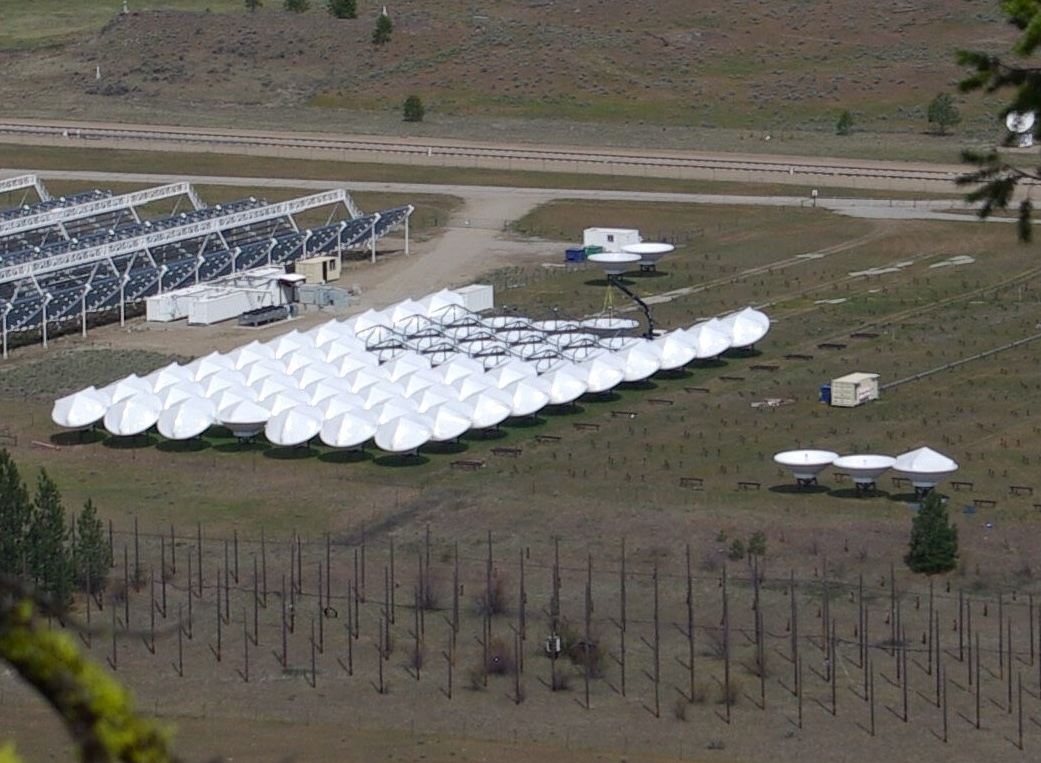
\includegraphics[width=0.8\linewidth]{plots/CHORD.jpeg}
      \par\medskip
      {\footnotesize The CHORD array, once complete, will consist of 512 6-meter dishes \cite{SPIEpaper}}
    \end{column}
  \end{columns}
\end{frame}

\section[RFI]{Radio Frequency Interference}
\subsection{Definition of RFI}
\begin{frame}{Definition of RFI}{}
  \begin{columns}[T]
    \begin{column}{0.5\linewidth}
      \begin{itemize}
        \item Radio frequency interference (RFI) consists of all non-astronomical radio signals that can contaminate astronomical observations.
        \item RRLs will only be detectable if there is no RFI present at the RRL transition frequency.
      \end{itemize}
    \end{column}
    \begin{column}{0.45\linewidth}
      \centering
      {\usebeamercolor[fg]{structure}Examples of RFI}
      \par\smallskip
      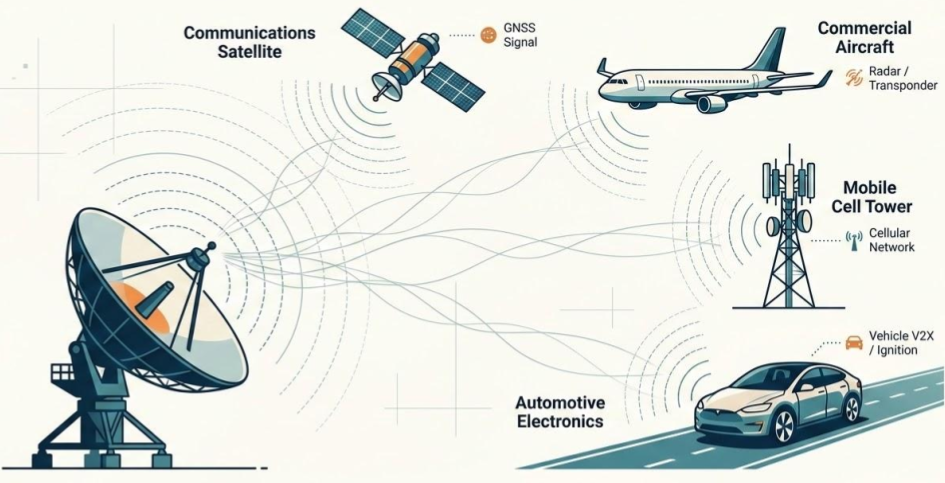
\includegraphics[width=1\linewidth]{plots/RFI_examples.png}
      \par\medskip
      {\footnotesize Sources of RFI include satellites, aircraft, mobile phones, and cars. \cite{RFI_image}}
    \end{column}
  \end{columns}
\end{frame}

\subsection{RFI Monitor}
\begin{frame}{RFI Monitor}{}
  \begin{columns}[T]
    \begin{column}{0.5\linewidth}
      \begin{itemize}
        \item The RFI monitor records radio signals from $0-2$ GHz.
      \end{itemize}
      \begin{enumerate}
        \item Complex voltages are measured and converted to power
        \[P = |V|^2 \sim \text{Exp}(2\sigma^2). \]
        \item Power is integrated over $N = 2500$ time samples
        \[P_N = \sum_{i=1}^{N} P_i \sim \text{Gamma}(N, 2\sigma^2).\]
      \end{enumerate}
    \end{column}
    \begin{column}{0.45\linewidth}
      \centering
      {\usebeamercolor[fg]{structure}DRAO RFI Monitor}
      \par\smallskip
      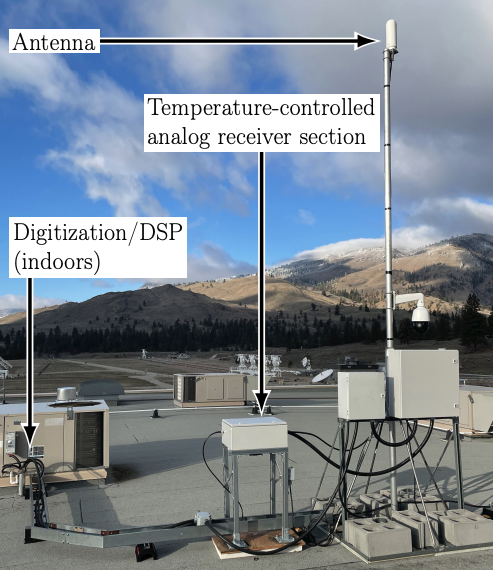
\includegraphics[width=0.7\linewidth]{plots/RFI_monitor.png}
      \par\medskip
      {\footnotesize The roof mounted DRAO RFI monitor \cite{bruceWidebandRFIMonitor2026}.}
    \end{column}
  \end{columns}
\end{frame}

\subsection{RFI Detection}
\begin{frame}{RFI Detection}{Spectral Kurtosis definition}
  \begin{columns}[T]
    \begin{column}{0.5\linewidth}
      \begin{itemize}
        \item System noise and astronomical signals are Gaussian distributed over time, while RFI is not.
        \item Spectral Kurtosis (SK) \cite{nitaGeneralizedSpectralKurtosis2010} is a measure of Gaussianity in a power timeseries.
        \item For a Gaussian voltage timeseries, the spectral kurtosis is 1.
      \end{itemize}
    \end{column}
    \begin{column}{0.5\linewidth}
      \centering
      {\usebeamercolor[fg]{structure}The generalized spectral kurtosis estimator:}
      \begin{align*}
          \text{let:} \quad S_1 &= \sum_{j=1}^{M} P_{N,j}, \quad S_2 = \sum_{j=1}^{M} P_{N,j}^2 \\[4pt]
          \widehat{SK} &= \frac{M N d + 1}{M - 1} \left( \frac{M S_2}{S_1^2} - 1 \right),
      \end{align*}
      {\footnotesize Where $P_{N}$ is the integrated power per frequency channel, $M$ is the number of integrated time samples, $Nd$ is the number of independent time samples per integration.}
    \end{column}
  \end{columns}
\end{frame}

\begin{frame}{RFI Detection}{Spectral Kurtosis Calibration}
  \begin{columns}[T]
    \begin{column}{0.5\linewidth}
      \begin{itemize}
        \item We used RFI free data from the RFI protected band of 1400-1430 MHz to calibrate the SK estimator.
        \item This is required since the RFI monitor does not obtain perfectly independent time samples, which biases the estimator.
        \item The calibrated shape parameter is found to be $Nd = 2500\cdot 15/16 \times 0.96$
      \end{itemize}
    \end{column}
    \begin{column}{0.5\linewidth}
      \centering
      {\usebeamercolor[fg]{structure}SK calibration}
      \par\smallskip
      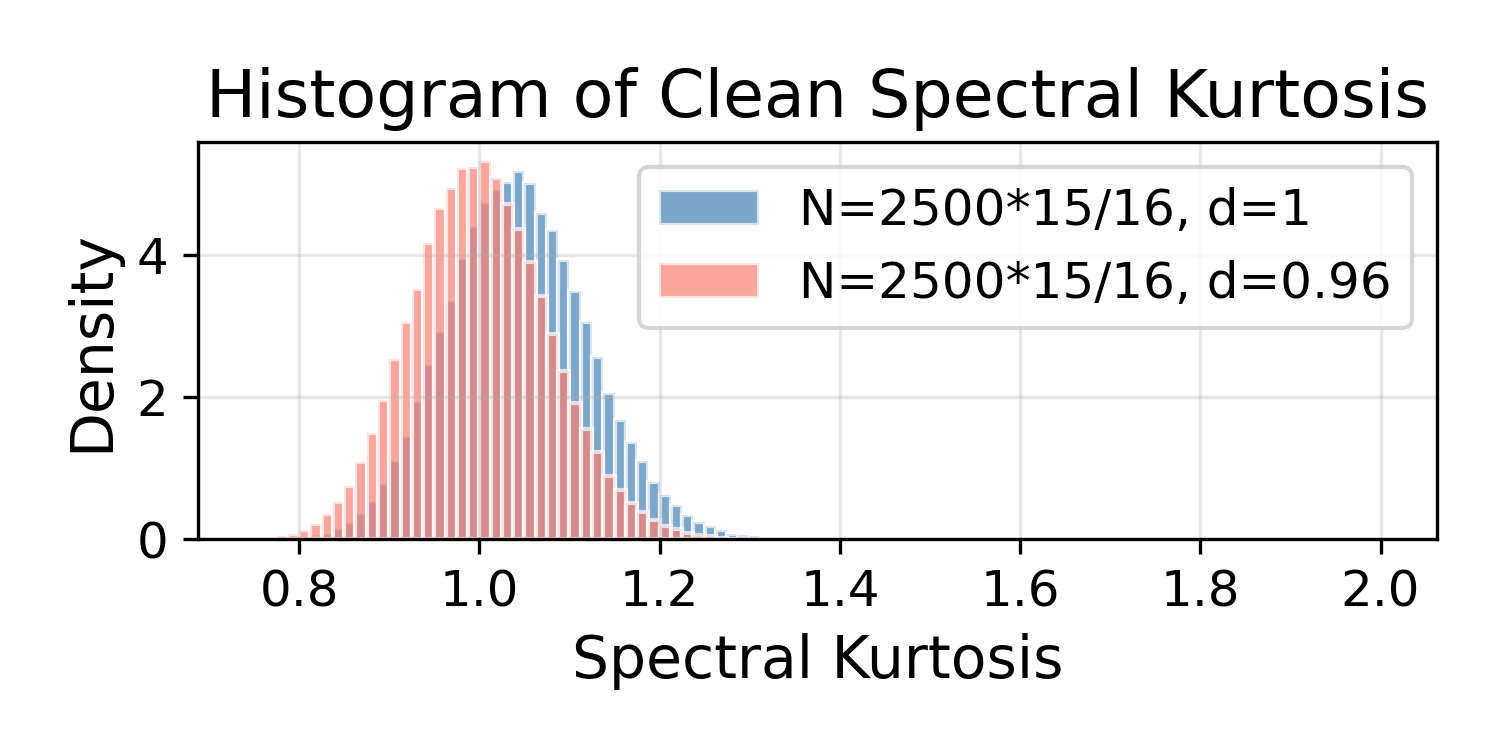
\includegraphics[width=1\linewidth]{../thesis/plots/rfi/hist_setting_sk_p.png}
      \par\medskip
      {\footnotesize The SK estimator (blue) is calibrated on clean data (red) to have a mode of exactly 1.}
    \end{column}
  \end{columns}
\end{frame}

\begin{frame}{RFI Detection}{Spectral Kurtosis RFI thresholds}
  \begin{columns}[T]
    \begin{column}{0.5\linewidth}
      \begin{itemize}
        \item The RFI-free SK distribution is simulated with $10^5$ Monte Carlo draws from $\texttt{Gamma}(Nd, 2\sigma^2)$.
        \item The observed SK in the clean 1400--1430 MHz band matches these simulations, confirming the band is RFI free.
        \item The simulated 0.1\% and 99.9\% quantiles set the detection thresholds: SK values outside them are flagged as RFI.
      \end{itemize}
    \end{column}
    \begin{column}{0.5\linewidth}
      \centering
      {\usebeamercolor[fg]{structure}Null SK distribution with RFI detection thresholds}
      \par\smallskip
      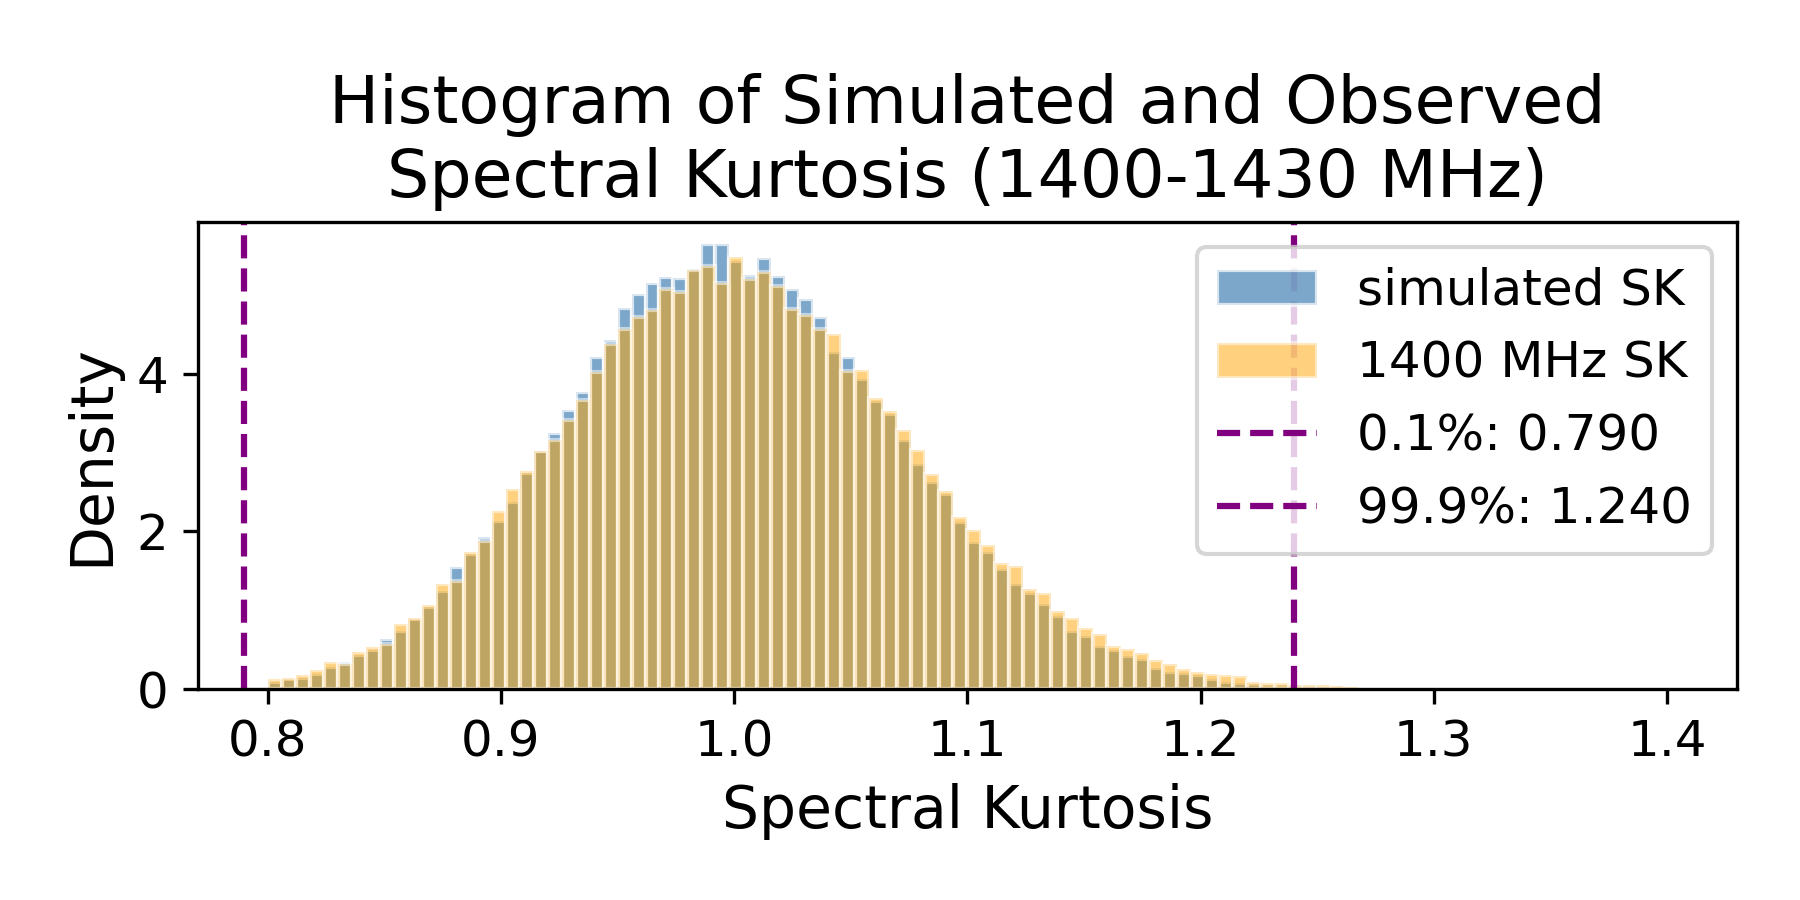
\includegraphics[width=1\linewidth]{../thesis/plots/rfi/spectral_kurtosis_all_time.png}
      \par\medskip
      {\footnotesize Simulated null SK distribution (blue) matches with observed non-RFI SK (red). RFI thresholds are taken as the 0.1\% and 99.9\% quantiles.}
    \end{column}
  \end{columns}
\end{frame}

\begin{frame}{RFI Detection}{SK flagging results}
  \begin{columns}[T]
    \begin{column}{0.5\linewidth}
      \centering
      {\usebeamercolor[fg]{structure}Power and SK on RFI spectrum}
      \par\smallskip
      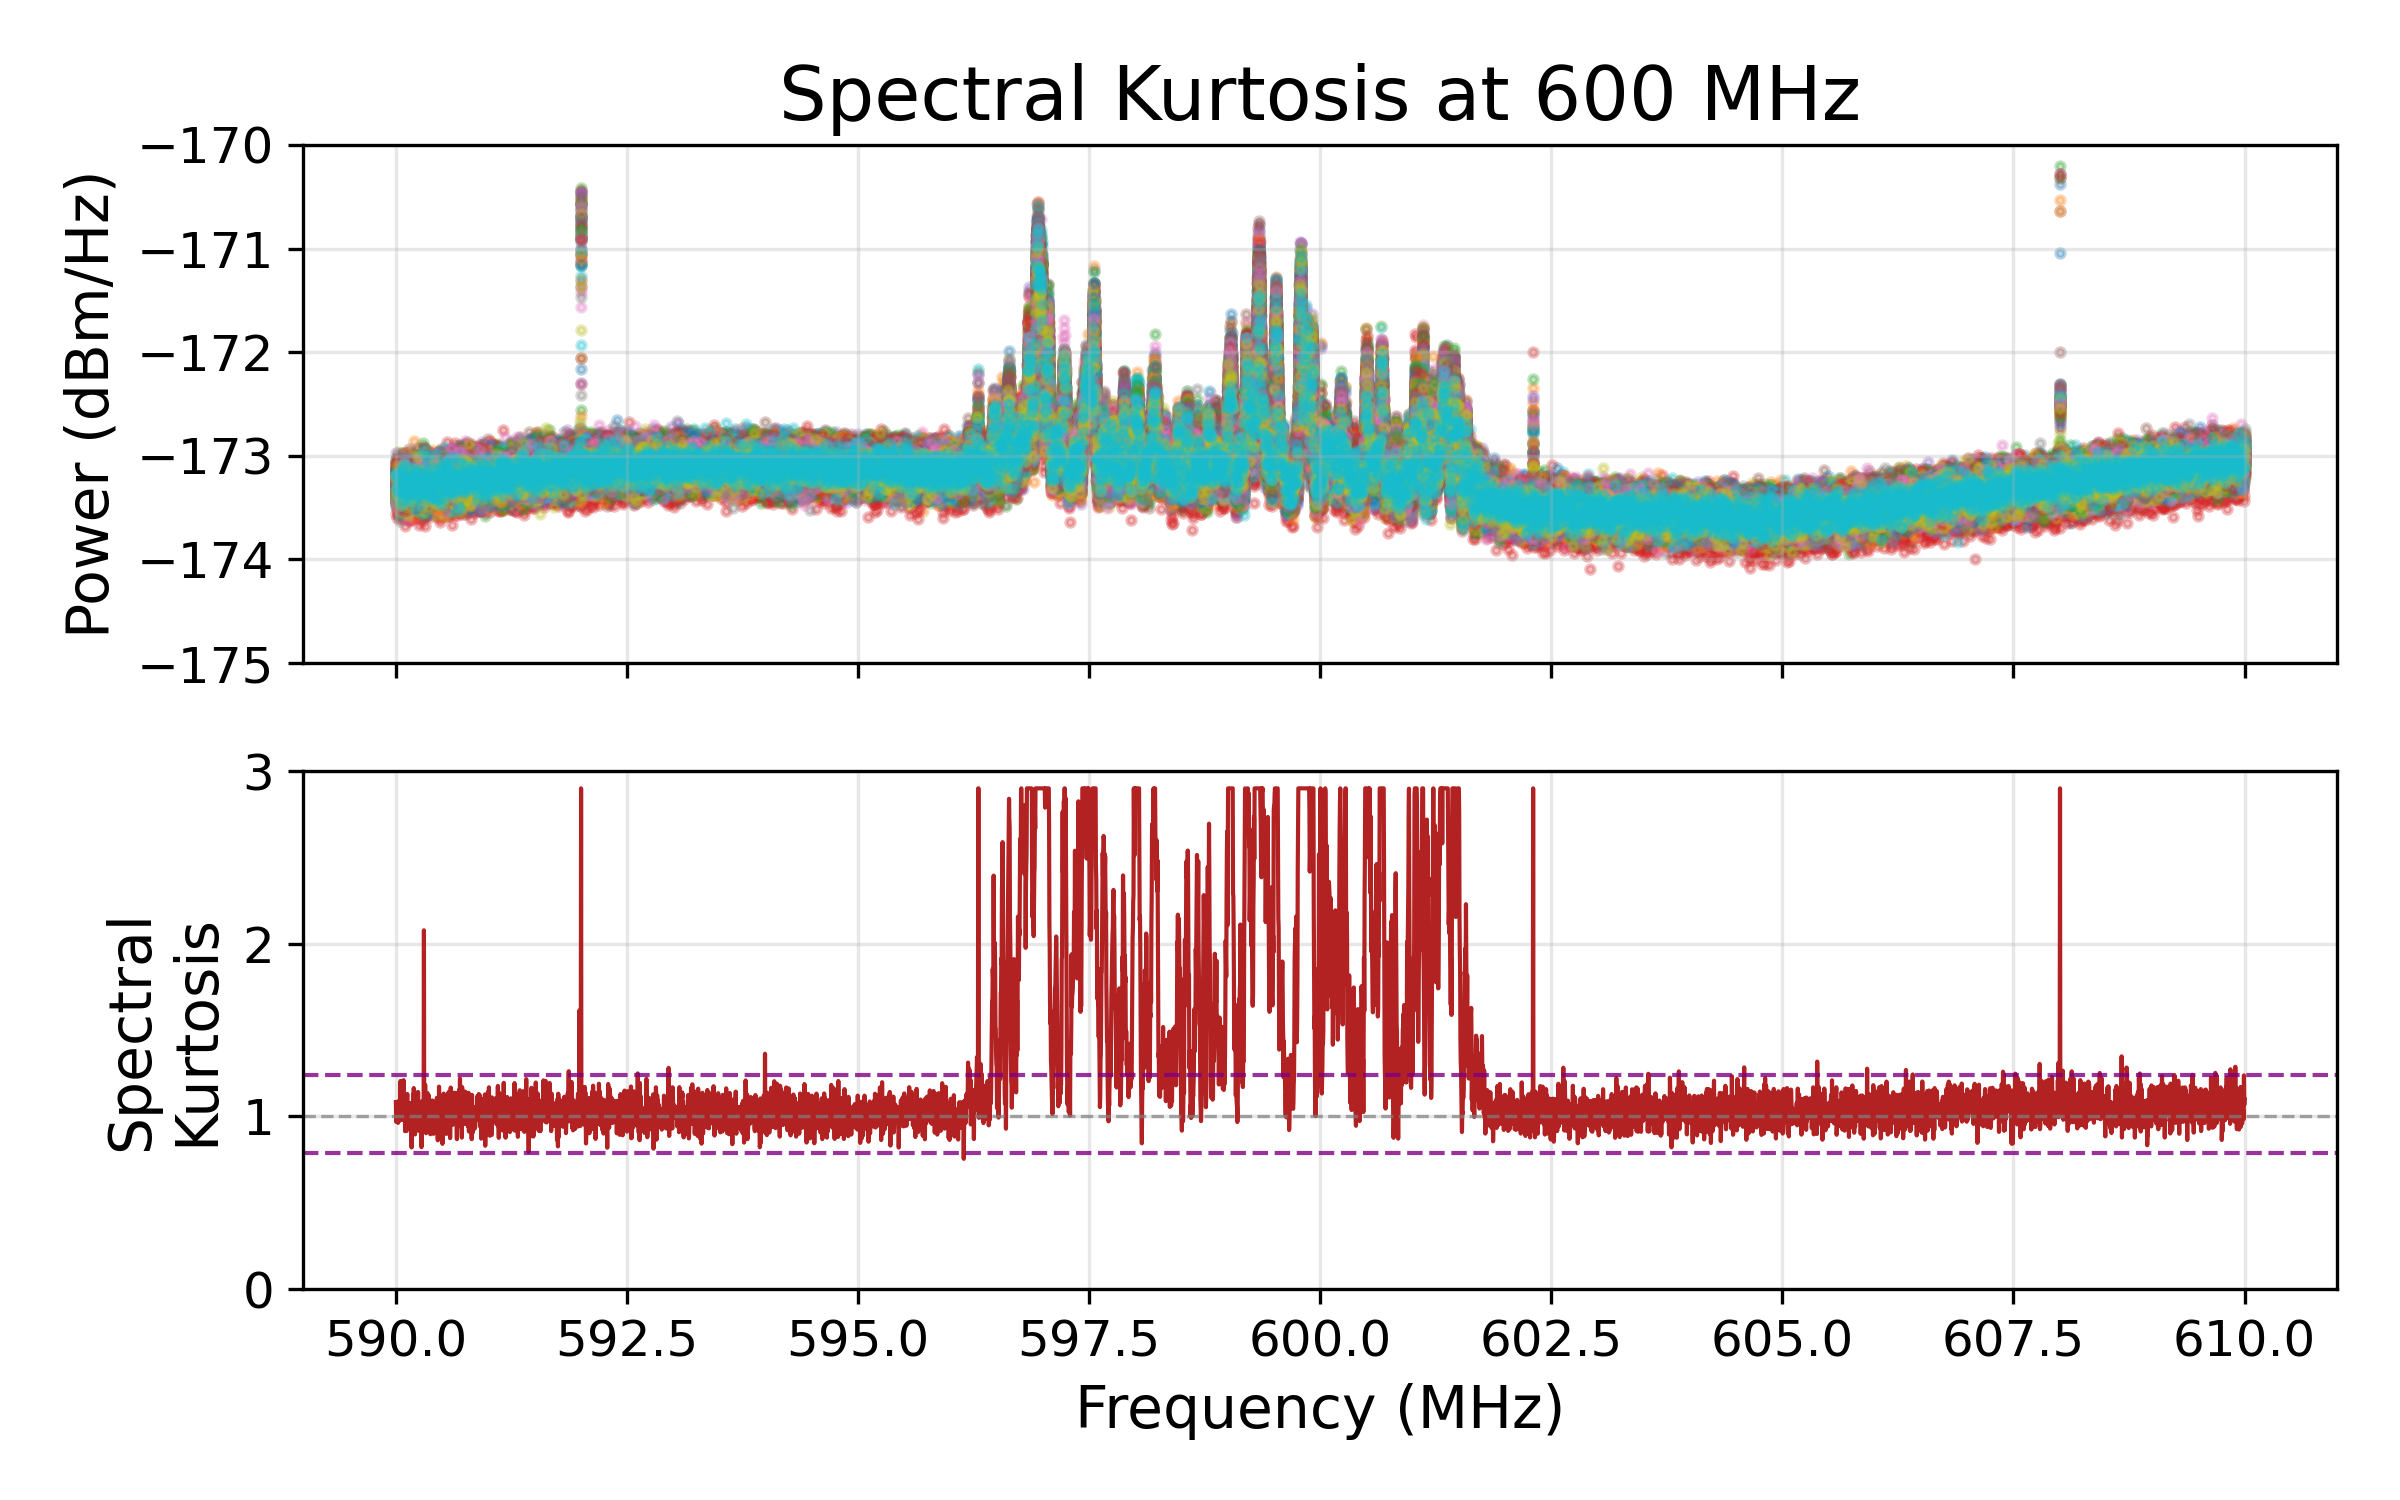
\includegraphics[width=1\linewidth]{../thesis/plots/rfi/600MHz_sample_SK.png}
      \par\medskip
      {\footnotesize SK (bottom plot) clearly shows RFI-affected spectrum present in the Power measurement (top).}
    \end{column}
    \begin{column}{0.5\linewidth}
      \centering
      {\usebeamercolor[fg]{structure}RFI flagging results, full CHORD band}
      \par\smallskip
      \includegraphics[width=1\linewidth]{../thesis/plots/rfi/RFI_flagged_spectrum.png}
      \par\medskip
      {\footnotesize RFI monitor power colored by SK RFI flagging results. In total 75.6\% of the CHORD band is found to be RFI free.}
    \end{column}
  \end{columns}
\end{frame}

\subsection{Line Characterization}
\begin{frame}{Line Characterization}{Gaussian weighted average around each RRL}
  \begin{columns}[T]
    \begin{column}{0.5\linewidth}
      \begin{itemize}
        \item For a line to be detectable, it should be mostly RFI free within $\pm 200 \text{ km/s}$.
        \item We compute a per line score as a Gaussian weighted average of the binary RFI labels centered at the rest frequency with a standard deviation of $\sigma_f = 100 \text{ km/s}$
      \end{itemize}
      \begin{align*}
        s = \frac{\sum_i w_i\, \text{RFI}_i}{\sum_i w_i},~~w_i = \exp\!\left(-\frac{(f_i - f_0)^2}{2\sigma_f^2}\right)
      \end{align*}
    \end{column}
    \begin{column}{0.5\linewidth}
      \centering
      {\usebeamercolor[fg]{structure}Clean Scores}
      \par\smallskip
      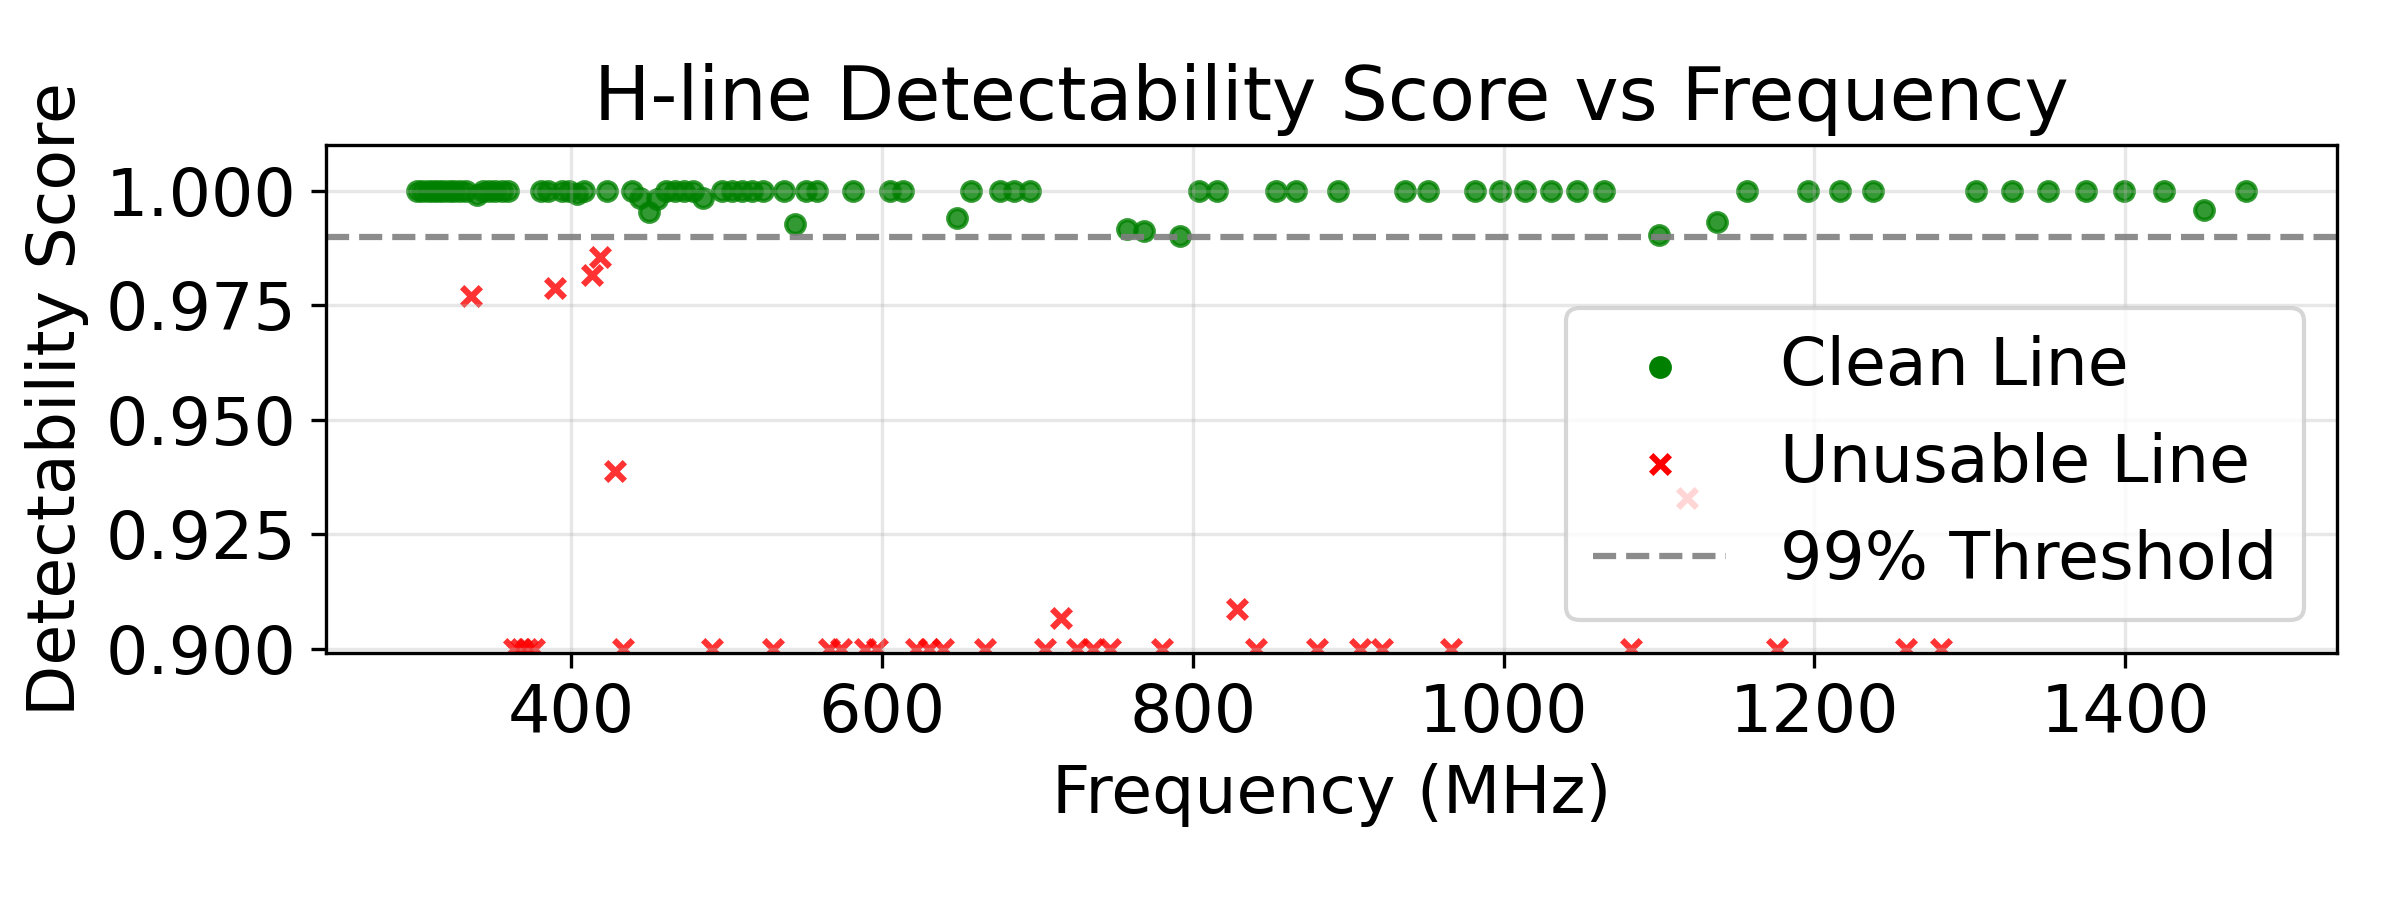
\includegraphics[width=1\linewidth]{../thesis/plots/rfi/h_line_clean_score.png}
      \par\medskip
      {\footnotesize Per line clean scores for all 116 Hn$\alpha$ RRLs in the CHORD band. Lines with a score $>0.99$ are considered detectable.}
    \end{column}
  \end{columns}
\end{frame}

\begin{frame}{Line Characterization}{Detectable Lines by Frequency Range}
  \centering
  {\usebeamercolor[fg]{structure}Detectable vs.\ RFI-contaminated Hn$\alpha$ RRLs}
  \par\medskip
  \begin{tabular}{lrr}
    \toprule
    \textbf{Frequency Range} & \textbf{Detectable} & \textbf{Contaminated} \\
    \textbf{(MHz)} & \textbf{Transitions} & \textbf{Transitions} \\
    \midrule
    300--470   & 29 & 10 \\
    470--800   & 23 & 16 \\
    800--1500  & 27 & 11 \\
    \midrule
    \textbf{Total} & \textbf{79} & \textbf{37} \\
    \bottomrule
  \end{tabular}
  \par\medskip
\end{frame}

\begin{frame}{Limitations}{}
\begin{itemize}
    \item CHORD is orders of magnitude more sensitive than the RFI monitor, signals that are not detectable by the RFI monitor may nonetheless impede CHORD.
    \item CHORD has a directional beam pointed upwards while the RFI monitor is most sensitive downwards and horizontally, RFI from overhead may be missed by the RFI monitor.
    \item This analysis is based on a single hour of RFI monitor data, which may not be representative of the long-term RFI environment.
    \item RFI changes over time, as new RFI sources emerge, spectrum currently free of RFI might become corrupted.
\end{itemize}
\end{frame}

\section{Sensitivity}
\subsection{Sensitivity Definitions}
\begin{frame}{Sensitivity Definitions}{Point Source Sensitivity}

  A telescope's sensitivity, choosing a signal-to-noise ratio (SNR) of 1, is equivalent to the root mean square (RMS) noise of the telescope.\\
  ~\\
  The point-source RMS noise follows the radiometer equation, which for dual polarization is given by
  \[
  \sigma_{\mathrm{RMS}}\,[\mathrm{Jy/beam}] = \frac{2k\,(T_{\mathrm{ant}}+T_{\mathrm{sky}})}{A_e\sqrt{2\,\Delta\nu\,\tau_{\mathrm{eff}}\,N(N-1)}}
  \]
  where $k$ is Boltzmann's constant, $T_{\mathrm{ant}}$ is the antenna temperature, $T_{\mathrm{sky}}$ is the sky temperature, $A_e$ is the effective area of a single dish, $\Delta\nu$ is the bandwidth, $\tau_{\mathrm{eff}}$ is the effective integration time, and $N$ is the number of dishes.
\end{frame}

\begin{frame}{Sensitivity Definitions}{Angular Resolution}
  The angular resolution is the smallest angular scale the telescope can resolve. It is defined as the full width at half maximum (FWHM) of the synthesized beam, which is the combined beam after correlating all pairs of dishes in the interferometer.\\
  ~\\
  The angular resolution of an interferometer is set by the longest baseline between two dishes ($D_{\mathrm{EW}}$ and $D_{\mathrm{NS}}$) and the observing wavelength ($\lambda$),
  \[
  \theta_{\mathrm{FWHM}} = \frac{\lambda}{D_{\mathrm{EW}}}, \quad \phi_{\mathrm{FWHM}} = \frac{\lambda}{D_{\mathrm{NS}}}.
  \]
  The beam solid angle is the area subtended by the synthesized beam,
  \[
  \Omega_s = \frac{\pi}{4\ln 2}\,\theta_{\mathrm{FWHM}}\,\phi_{\mathrm{FWHM}}.
  \]
\end{frame}


\begin{frame}{Sensitivity Definitions}{Brightness Temperature Sensitivity}

  Brightness temperature sensitivity, is a measure of the telescope's ability to detect extended sources. It is obtained by dividing the point-source RMS noise by the beam solid angle, and converting from Jy/beam to K by applying the Rayleigh-Jeans limit.\\
  ~\\
  \[
  \sigma_T\,[\mathrm{K}] = \frac{\sigma_{\mathrm{RMS}}}{\Omega_s}\,
\frac{c^2}{2k\nu^2}
  \]
\end{frame}

\subsection{Sensitivity Maps}
\begin{frame}{Sensitivity Maps}{Intrinsic CHORD Brightness Temperature Sensitivity}
  \begin{columns}[T]
    \begin{column}{0.5\linewidth}
      \begin{itemize}
        \item Low Frequency is better.\\
        A larger primary beam means more integration time per source.
        \item High declination is better.\\
        Sources transit slower, allowing more integration time per observing day.
      \end{itemize}
    \end{column}
    \begin{column}{0.5\linewidth}
      \centering
      {\usebeamercolor[fg]{structure}Intrinsic CHORD Sensitivity}
      \par\smallskip
      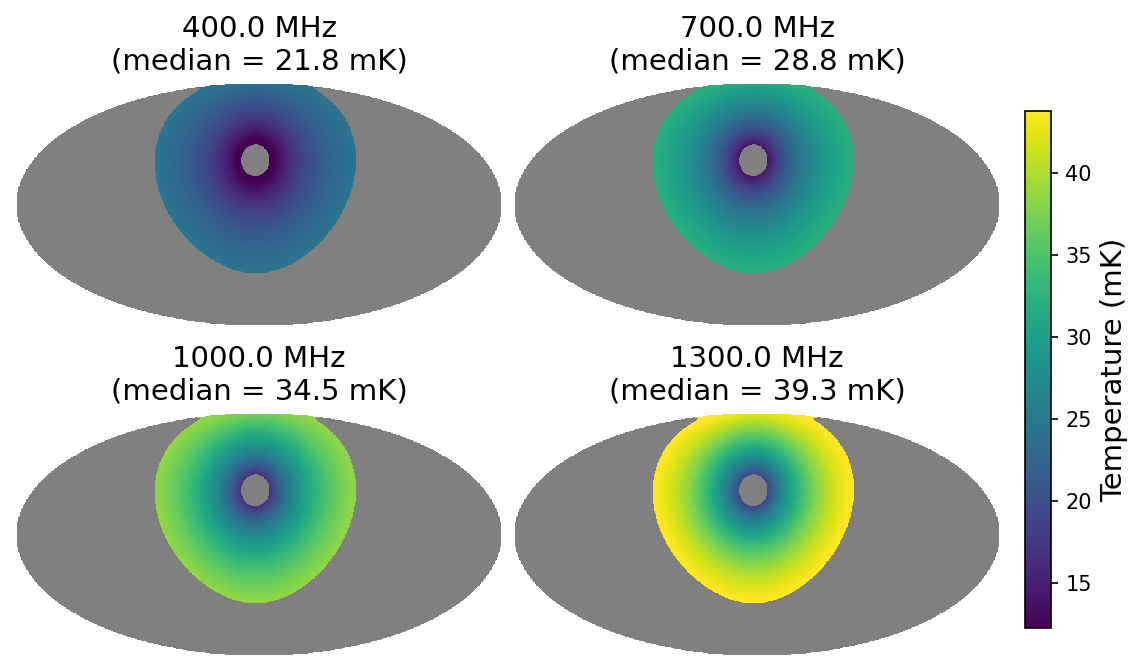
\includegraphics[width=1\linewidth]{../thesis/plots/sensitivity/system_only_noise.png}
      \par\medskip
      {\footnotesize Intrinsic CHORD brightness temperature sensitivity over the CHORD observing range plotted in galactic coordinates.}
    \end{column}
  \end{columns}
\end{frame}

\begin{frame}{Sensitivity Maps}{Radio Background}
  \begin{columns}[T]
    \begin{column}{0.5\linewidth}
      \begin{itemize}
      \item Recall that the point-source RMS is proportional to the antenna temperature ($T_{\mathrm{ant}}= 30 \,\mathrm{K}$) and the sky temperature ($T_{\mathrm{sky}}$):
      \[
      \sigma_{\mathrm{RMS}} = \frac{2k\,(T_{\mathrm{ant}}+T_{\mathrm{sky}})}{A_e\sqrt{2\,\Delta\nu\,\tau_{\mathrm{eff}}\,N(N-1)}}
      \]
      \item Radio background is generally highest at low frequency and along the galactic plane.
      \end{itemize}
    \end{column}
    \begin{column}{0.5\linewidth}
      \centering
      {\usebeamercolor[fg]{structure}Radio Background}
      \par\smallskip
      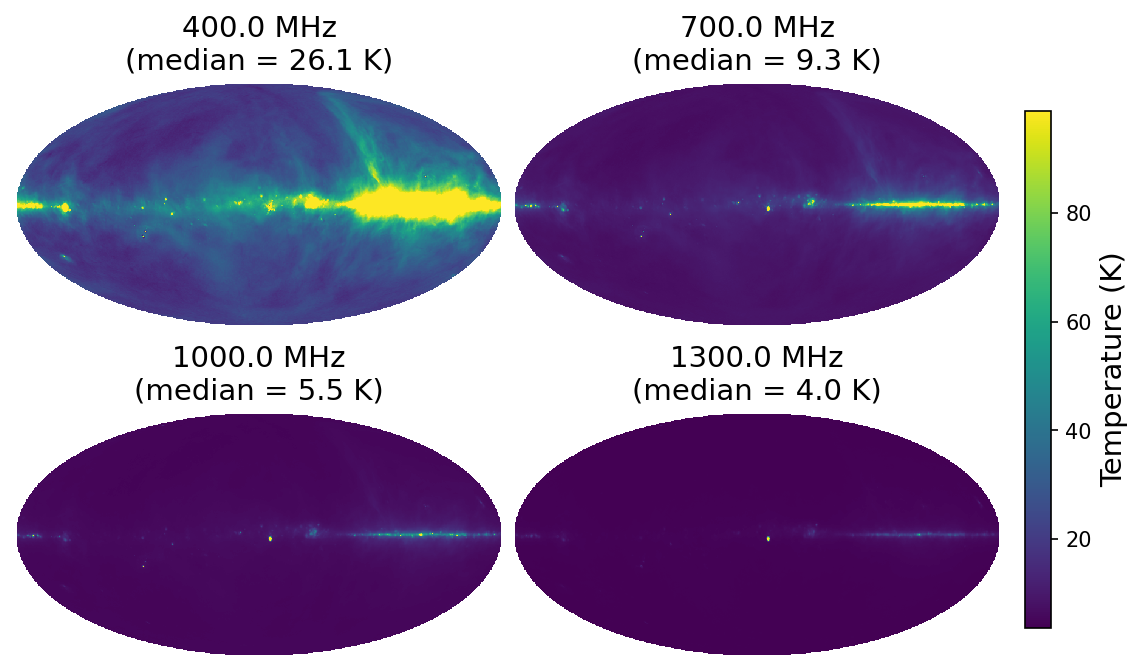
\includegraphics[width=1\linewidth]{../thesis/plots/sensitivity/background_only.png}
      \par\medskip
      {\footnotesize Radio Background obtained from the 2016 Global Sky Model \cite{zhengImprovedModelDiffuse2017}.}
    \end{column}
  \end{columns}
\end{frame}

\begin{frame}{Sensitivity Maps}{Total Sensitivity}
  \begin{columns}[T]
    \begin{column}{0.5\linewidth}
      \begin{itemize}
        \item Total CHORD sensitivity including radio background
        \item Sensitivity is highly spatially and frequency dependent.
      \end{itemize}
    \end{column}
    \begin{column}{0.5\linewidth}
      \centering
      {\usebeamercolor[fg]{structure}Total CHORD Sensitivity}
      \par\smallskip
      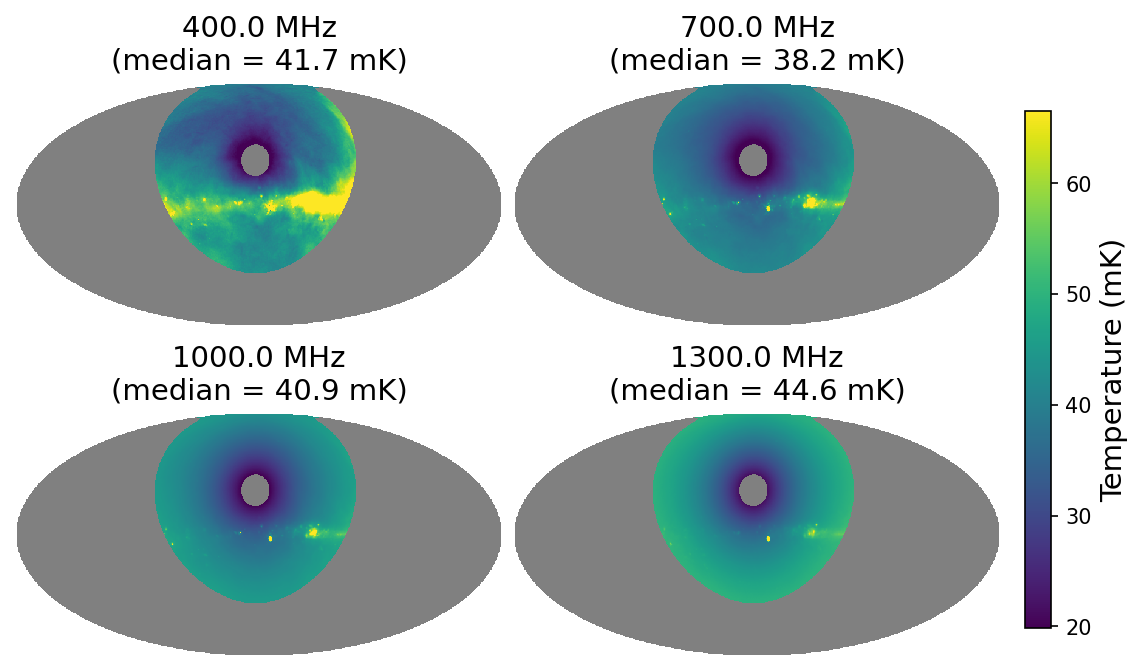
\includegraphics[width=1\linewidth]{../thesis/plots/sensitivity/total_noise.png}
      \par\medskip
      {\footnotesize Total CHORD brightness temperature sensitivity over the CHORD observing range.}
    \end{column}
  \end{columns}
\end{frame}

\begin{frame}{Limitations}{}
  \begin{itemize}
    \item The system temperature is assumed to be constant at 30 K, but in reality it varies with frequency.
    \item The radio background from the 2016 Global Sky Model is obtained by modeling values between the 408 MHz Haslam map and the 1.42 GHz Reich map, it may not be perfectly accurate at all frequencies and the angular resolution is limited to roughly 1 degree (56 arcminutes).
  \end{itemize}
\end{frame}

\section[SNR \& Smoothing]{Line Strength and Smoothing}
\subsection{Line Strength}
\begin{frame}{Line Strength}{}
  Emission intensity of an RRL is a function of the physical quantities of the ISM and the transition frequency. Peak line strength is given by \cite{andersonGBTDiffuseIonized2021} as
  \begin{equation*}
    \left( \frac{T_L}{\text{K}} \right) \backsimeq 3076~\left(\frac{T_e}{\text{K}}\right)^{-3/2}\left(\frac{EM}{\text{pc cm}^{-6}}\right) \left(\frac{\nu_0}{\text{GHz}}\right)^{-1} \left(\frac{\Delta V}{\text{km s}^{-1}} \right)^{-1} \Delta n M_{\Delta n},
    \label{eq:line_intensity}
  \end{equation*}

where:
\begin{itemize} 
  \item $T_e$, the electron temperature, $EM$, the emission measure, and $\Delta V$, the line width, are physical quantities of the ISM. 
  \item $\Delta n M_{\Delta n}$ is a quantum mechanical factor that is constant for all $n\alpha$ transitions. 
  \item $\nu_0$ is the rest frequency of the transition. \\
  \item \textbf{Meaning Line strength increases at lower frequencies.}
\end{itemize}
\end{frame}

\subsection{SNR by Region}
\begin{frame}{SNR by region}{Selected Regions}
  \begin{columns}[T]
    \begin{column}{0.5\linewidth}
      \begin{itemize}
        \item Signal is frequency dependent.\\
        It increases at low frequency.
        \item Sensitivity is frequency dependent.\\
        \item Sensitivity is spatially dependent.\\
        \item We select three locations to analyse which lines are most important within each region.
      \end{itemize}
    \end{column}
    \begin{column}{0.5\linewidth}
      \centering
      {\usebeamercolor[fg]{structure}Map of regions for further analysis}
      \par\smallskip
      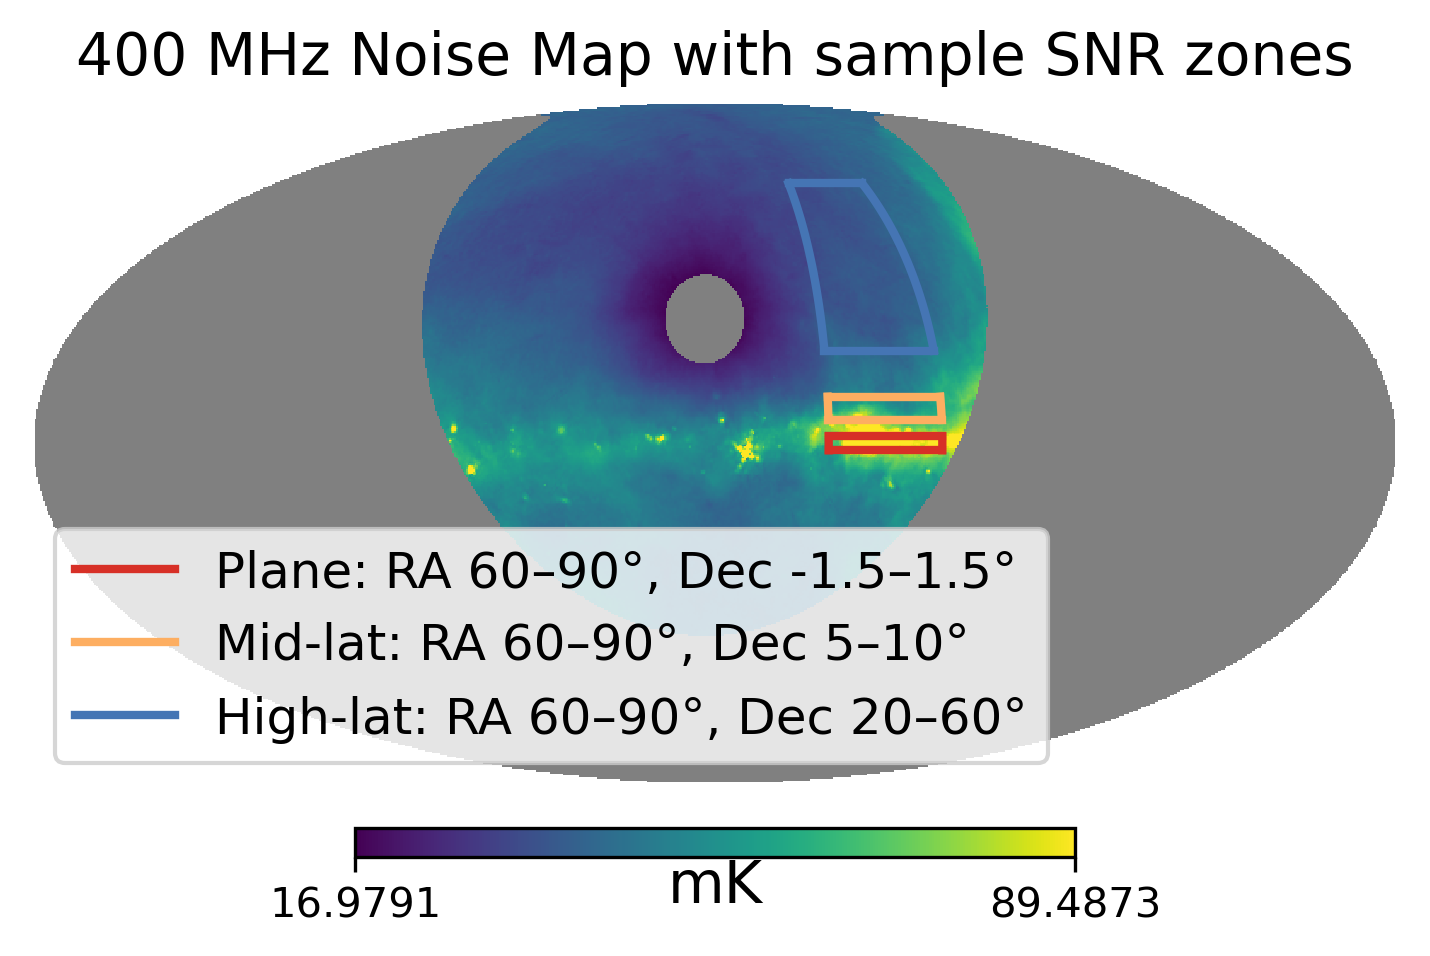
\includegraphics[width=0.8\linewidth]{../thesis/plots/sensitivity/snr_locations.png}
      \par\medskip
      {\footnotesize We take the median sensitivity over each region, Galactic plane, mid-latitude, and high-latitude.}
    \end{column}
  \end{columns}
\end{frame}

\begin{frame}{SNR by region}{Native SNR per RRL}
  \begin{columns}[T]
    \begin{column}{0.5\linewidth}
      \begin{itemize}
        \item Native SNR is best for low frequency RRLs.
      \end{itemize}
      \par\smallskip
      \vfill
      \centering
      {\usebeamercolor[fg]{structure}Native resolution}
      \par\smallskip
      \begin{tabular}{@{}lcc@{}}
        \toprule
        & \textbf{300 MHz} & \textbf{1.5 GHz} \\
        \midrule
        Angular Res. & $21'$              & $4.2'$ \\
        Velocity Res. & $5\ \mathrm{km\,s^{-1}}$ & $1\ \mathrm{km\,s^{-1}}$ \\
        \bottomrule
      \end{tabular}
      \par\medskip
      \begin{itemize}
        \item Low frequency has worse angular and velocity resolution.
      \end{itemize}
    \end{column}
    \begin{column}{0.5\linewidth}
      \centering
      {\usebeamercolor[fg]{structure}SNR by region, using native resolutions}
      \par\smallskip
      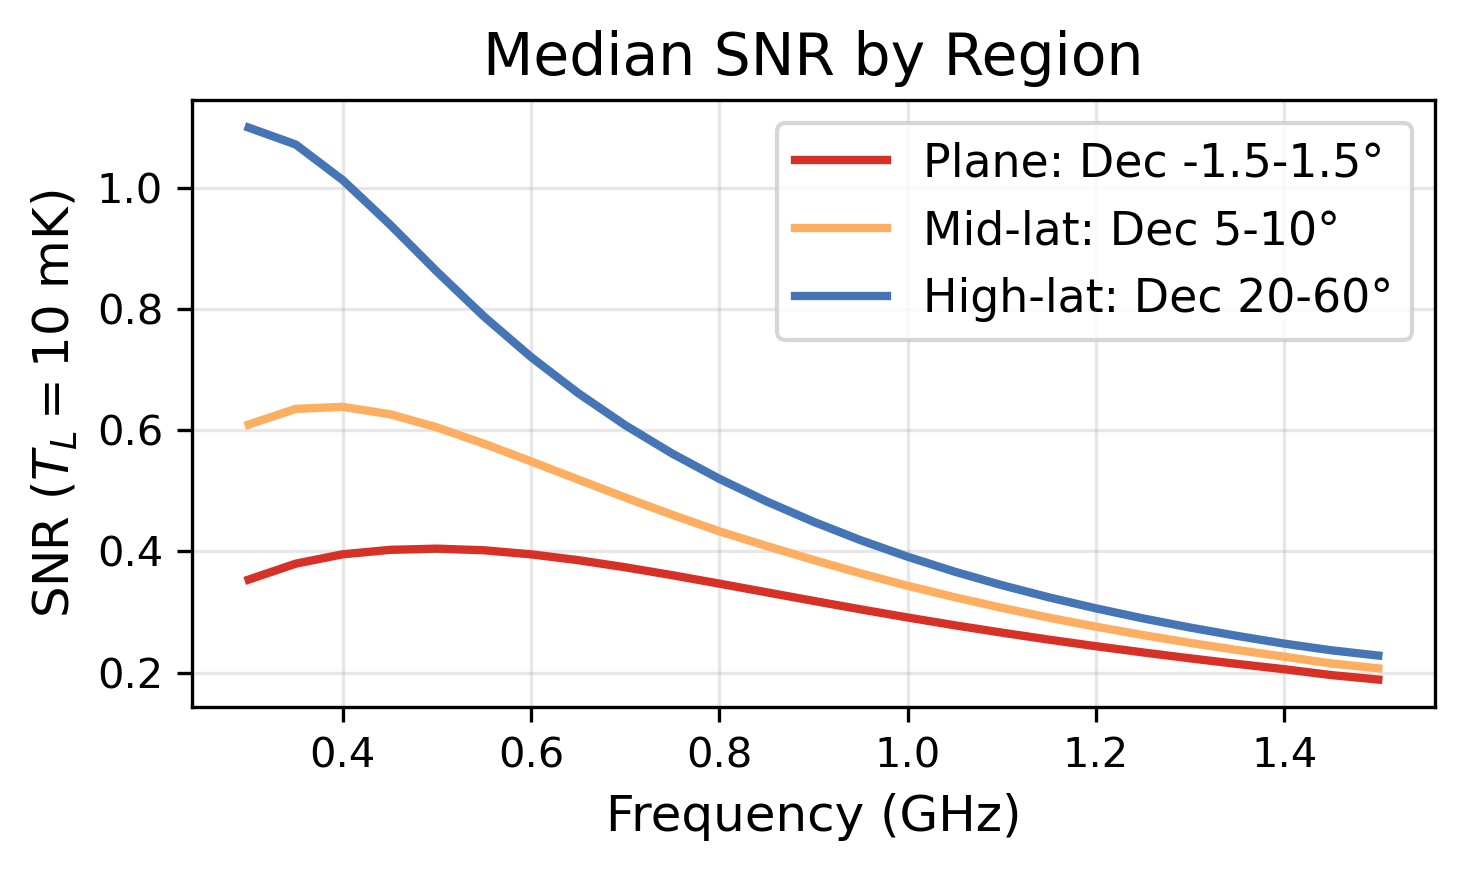
\includegraphics[width=1\linewidth]{../thesis/plots/sensitivity/snr_by_region.png}
      \par\medskip
      {\footnotesize Native SNR per RRL for each region, using the median sensitivity over each region.}
    \end{column}
  \end{columns}
\end{frame}

\begin{frame}{SNR by region}{SNR with smoothing}
  \begin{columns}[T]
    \begin{column}{0.5\linewidth}
      \begin{itemize}
        \item Each line sensitivity is computed for a 5 km s$^{-1}$ velocity resolution.
        \item Each line is smoothed to 22 arcminute angular resolution by treating each native beam as an independent sample of the larger smoothed beam.\\
        \[
        N = \frac{\Omega_{\mathrm{smoothed}}}{\Omega_{\mathrm{native}}}
        \]
        \[
        \sigma_T [\text{smoothed}] = \frac{\sigma_T [\text{native}]}{\sqrt{N}}
        \]

      \end{itemize}
    \end{column}
    \begin{column}{0.5\linewidth}
      \centering
      {\usebeamercolor[fg]{structure}SNR by region, after smoothing}
      \par\smallskip
      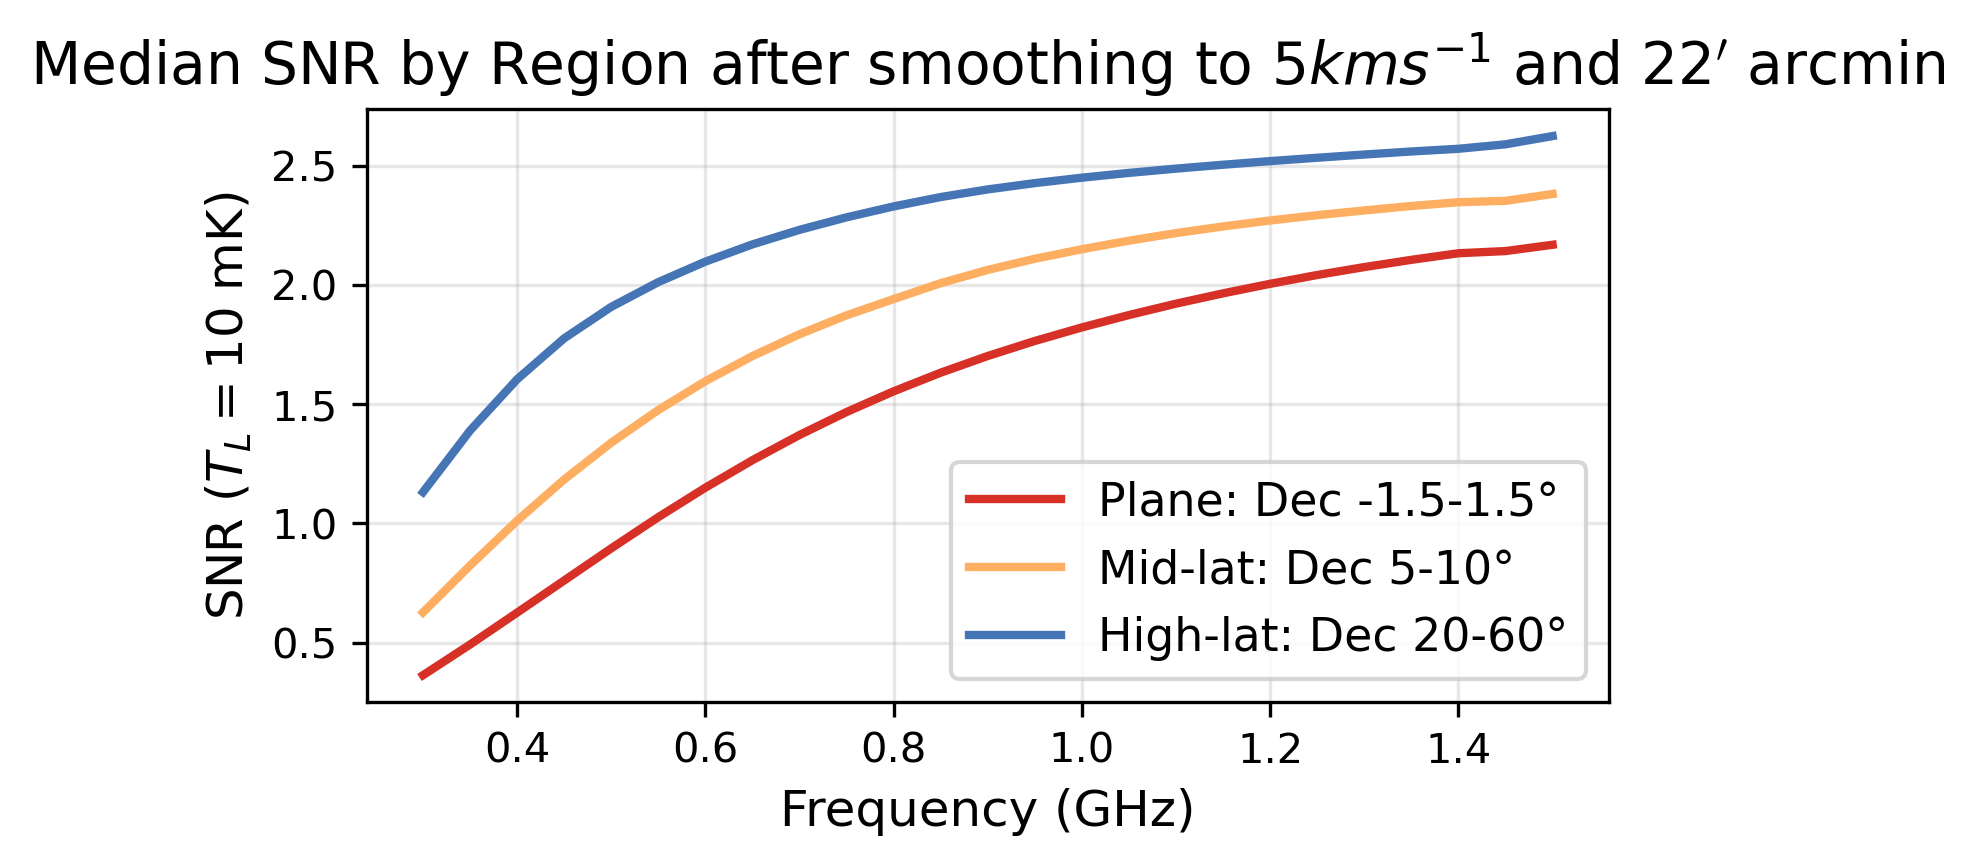
\includegraphics[width=1\linewidth]{../thesis/plots/sensitivity/smoothed_snr_by_region.png}
      \par\medskip
      {\footnotesize Smoothed SNR shows that high frequency RRLs now have the best per line SNR levels.}
    \end{column}
  \end{columns}
\end{frame}

% \begin{frame}{Stacking}{}
%   \begin{columns}[T]
%     \begin{column}{0.5\linewidth}
%       \begin{itemize}
%         \item RRLs of different frequencies are all produced by the same underlying physical quantities; gas temperature and density.
%         \item Measurement uncertainty is reduced by averaging signal from multiple RRLs.
%         \item Inverse-variance weighting is used to combine signals having different SNR levels.
%       \end{itemize}
%     \end{column}
%     \begin{column}{0.5\linewidth}
%       \centering
%       {\usebeamercolor[fg]{structure}Inverse-variance weighted average:}
%       \par\smallskip
%       \begin{equation*}
%         \hat{\mu} = \frac{\sum_i^N x_i w_i }{\sum_i^N w_i}, \quad \text{Var}(\hat{\mu}) = \frac{1}{\sum_i^N w_i},
%       \end{equation*}
%       \begin{equation*}
%         w_i = \frac{1}{\sigma_i^2},
%       \end{equation*}
%       \begin{equation*}
%         \text{SNR} = \frac{\hat{\mu}}{\sqrt{\text{Var}(\hat{\mu})}} = \frac{\sum_i^N x_i w_i}{\sqrt{\sum_i^N w_i}}.
%       \end{equation*}
%       \par\medskip
%       {\footnotesize Combined signal ($\hat{\mu}$), uncertainty ($\text{Var}(\hat{\mu})$) and SNR after stacking $N$ lines.}
%     \end{column}
%   \end{columns}
% \end{frame}

\begin{frame}{Limitations}{}
  \begin{itemize}
    \item Using the median sensitivity over each region ignores that H II regions have strong background emission, radio background is likely underestimated in this analysis compared to the actual locations of interest.
    \item The frequency bandwidths can't truly be set for each line but are instead smoothed in post-processing.
    \item True angular resolution smoothing such as \cite{andersonGBTDiffuseIonized2021} and \cite{liuSurveyIonizedGas2019} apply a Gaussian kernel over the native resolution maps, this analysis uses a boxcar average and assumes fully independent samples.
  \end{itemize}
\end{frame}

\section[SIGGMA]{Detection of SIGGMA Results}
\begin{frame}{CHORD detection of SIGGMA Results}{SIGGMA range}
  The Survey of Ionized Gas in the Galaxy Made with the Arecibo telescope (SIGGMA) made 427 RRL detections in the inner Galaxy region 32$^\circ~\leq~\ell~\leq~70^\circ$.\\
  \par\medskip
  \begin{columns}[T]
    \begin{column}{0.5\linewidth}
      \centering
      {\usebeamercolor[fg]{structure}SIGGMA survey covered by CHORD}
      \par\smallskip
      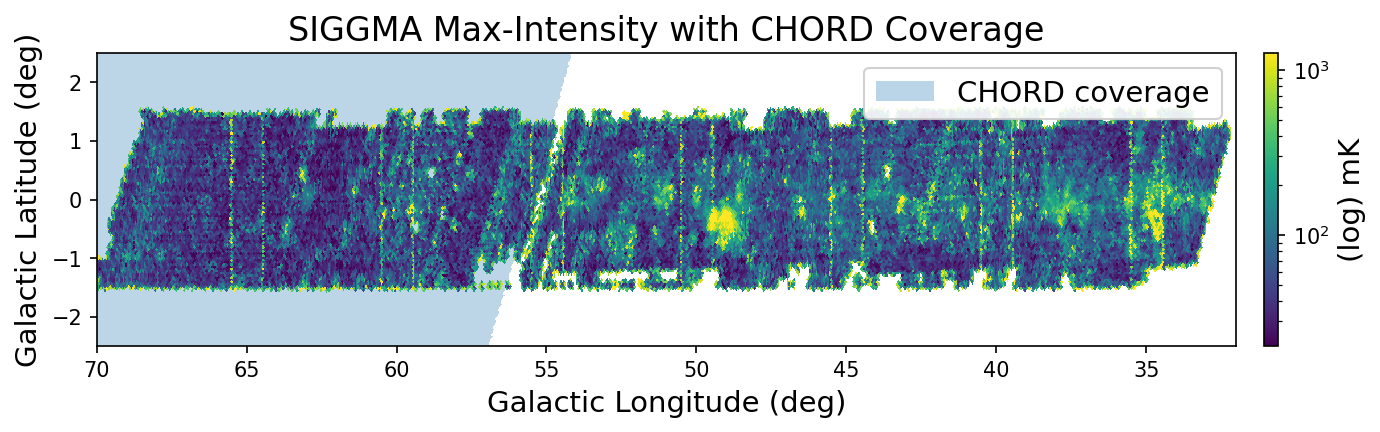
\includegraphics[width=1\linewidth]{../thesis/plots/siggma/siggma_with_chord_coverage.png}
      \par\medskip
      {\footnotesize CHORD only covers from $\sim 55^\circ~\leq~\ell~\leq~70^\circ$ which encompases 26 RRL detections.}
    \end{column}
    \begin{column}{0.5\linewidth}
      \centering
      {\usebeamercolor[fg]{structure}H II regions on CHORD sensitivity map}
      \par\smallskip
      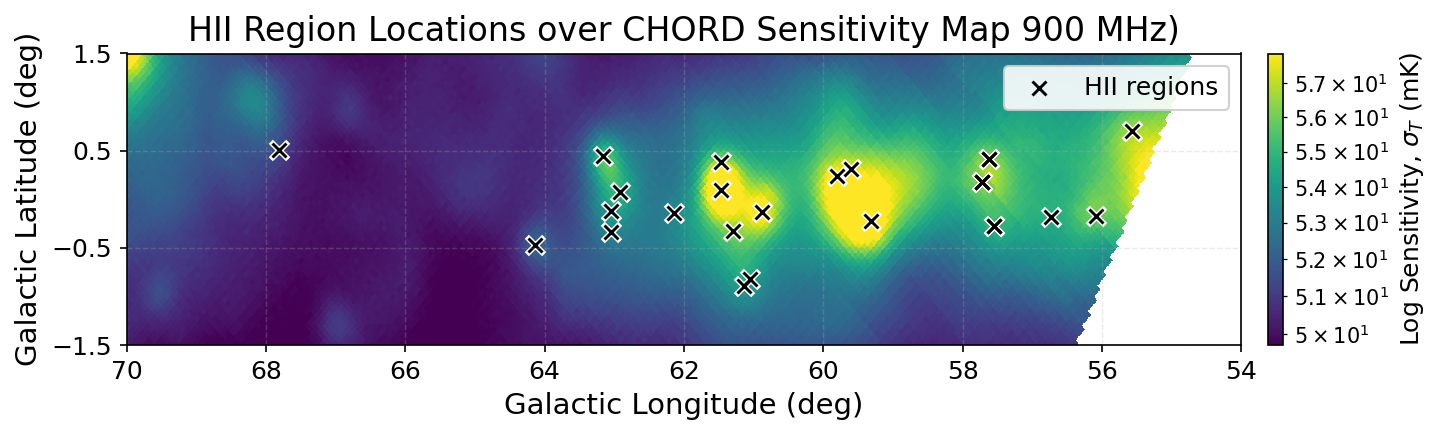
\includegraphics[width=1\linewidth]{../thesis/plots/siggma/hii_regions_over_chord_sensitivity.png}
      \par\medskip
      {\footnotesize The CHORD sensitivity at 900 MHz overlaid by the SIGGMA detections showing that H II regions mostly occur in high background regions.}
    \end{column}
  \end{columns}
\end{frame}

\begin{frame}{CHORD detection of SIGGMA Results}{SNR per smoothing level}
  \begin{columns}[T]
    \begin{column}{0.5\linewidth}
      \begin{itemize}
        \item SNR per detection is calculated by scaling the SIGGMA result to the given line frequency and dividing by the CHORD sensitivity at the detection location.
        \item High frequency lines offer the best SNR after smoothing to a common angular and velocity resolution.
        \item The number of lines to include depends on the angular resolution goal.
      \end{itemize}
    \end{column}
    \begin{column}{0.5\linewidth}
      \centering
      {\usebeamercolor[fg]{structure}SNR of SIGGMA detections after smoothing}
      \par\smallskip
      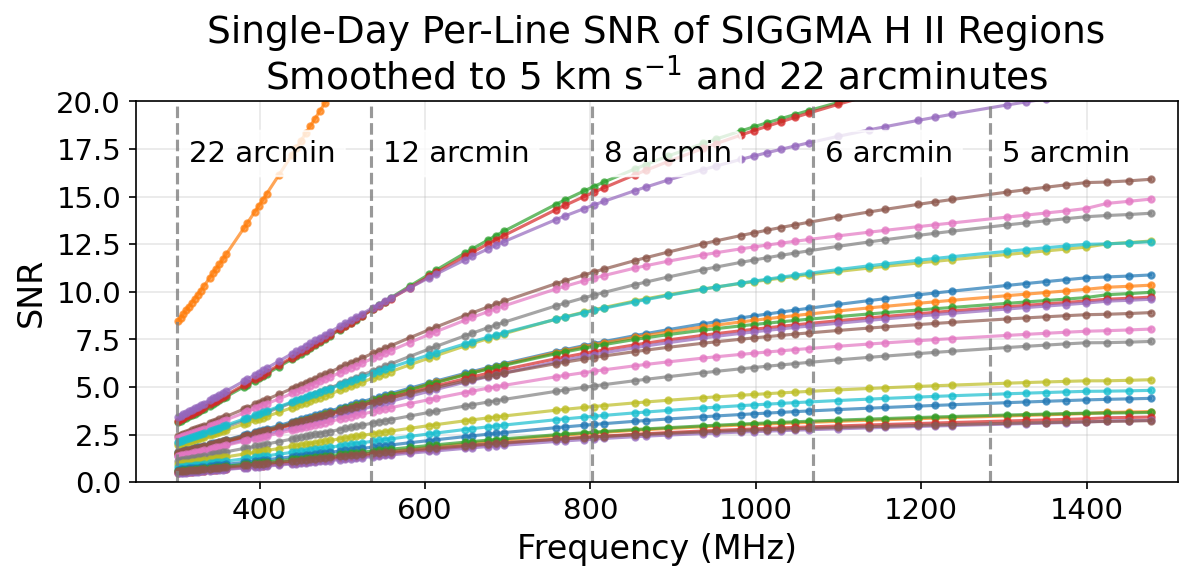
\includegraphics[width=1\linewidth]{../thesis/plots/siggma/SNR_per_SIGGMA_line_smoothed.png}
      \par\medskip
      {\footnotesize Fraction of lines to include depending on the angular smoothing level.}
    \end{column}
  \end{columns}
\end{frame}

\begin{frame}{CHORD detection of SIGGMA Results}{Smoothed SNR of each detection}
  \centering
  {\usebeamercolor[fg]{structure}Stacked SNR per H\,\textsc{ii} region, one observing day}
  \par\medskip
  \begin{tabular}{l c c c c}
    \toprule
    Order & Name & SNR $5'$ & SNR $6'$ & SNR $8'$ \\
    \midrule
    1 & G063.164+00.449 & $85.04 \pm 4.97$ & $130.52 \pm 7.63$ & $222.38 \pm 13.00$ \\
    2 & G061.473+00.094 & $41.86 \pm 3.23$ & $63.49 \pm 4.90$ & $105.47 \pm 8.14$ \\
    3 & G059.796+00.241 & $14.70 \pm 1.35$ & $22.45 \pm 2.06$ & $37.98 \pm 3.48$ \\
    $\vdots$ & $\vdots$ & $\vdots$ & $\vdots$ & $\vdots$ \\
    25 & G057.715+00.173 & $2.02 \pm 0.20$ & $3.11 \pm 0.31$ & $5.32 \pm 0.53$ \\
    26 & G062.142-00.144 & $2.03 \pm 0.31$ & $3.13 \pm 0.49$ & $5.42 \pm 0.84$ \\
    \bottomrule
  \end{tabular}
  \par\medskip
  {\footnotesize Smoothing to $5'$, $6'$, $8'$ stacks 8, 14, and 27 lines respectively.}
\end{frame}

\begin{frame}{Limitations}
  \begin{itemize}
    \item The radio background is estimated from the 2016 Global Sky Model which is limited to 56 arcminute resolution, this may underestimate the background at the precise H II locations, causing the SNR levels to be overstated.
    \item Some of the lines assumed clean in the RFI analysis may be contaminated by RFI, which would reduce the the stackable lines per smoothing threshold.
  \end{itemize}
\end{frame}

\section*{References}
\begin{frame}[allowframebreaks]{References}
  \footnotesize
  \bibliographystyle{apj}
  \bibliography{references}
\end{frame}
\end{document}

